\documentclass[english, aspectratio=169]{beamer}
% english is for the language used in standard texts (figures, tables etc)
% aspectratio of 16:9 or set it for more old school to 4:3 (without the ':')

% ---------------------------------------------------------------------------- %
% Load base preamble
% ---------------------------------------------------------------------------- %
\usepackage{import}
\subimport{./preamble/}{beamer.tex}

% ---------------------------------------------------------------------------- %
% Local settings
% ---------------------------------------------------------------------------- %
\newcommand{\B}[0]{\ensuremath{\mathbb{B}}}

\newcommand{\scan}[1]{\text{scan}(#1)}
\newcommand{\sort}[1]{\text{sort}(#1)}

\newcommand{\triple}[3]{\ensuremath{(#1, #2, #3)}}
\renewcommand{\arc}[3]{\ensuremath{#1 \xrightarrow{_{#2}} #3}}

% Citation-like footnotes: https://tex.stackexchange.com/a/333024
\makeatletter
% Default:
% \def\@makefnmark{\hbox{\@textsuperscript{\normalfont\@thefnmark}}}
\renewcommand{\@makefnmark}{\makebox{\normalfont[\@thefnmark]}}
\makeatother

% Horizontal legends: https://tex.stackexchange.com/a/101578
% argument #1: any options
\makeatletter
\newenvironment{customlegend}[1][]{%
  \begingroup
  % inits/clears the lists (which might be populated from previous
  % axes):
  \pgfplots@init@cleared@structures
  \pgfplotsset{#1}%
}{%
  % draws the legend:
  \pgfplots@createlegend
  \endgroup
}%

% makes \addlegendimage available (typically only available within an
% axis environment):
\def\addlegendimage{\pgfplots@addlegendimage}
\makeatother

% colors
\colorlet{adiar-skip_transpose}{green!50!cyan!80!black}
\colorlet{adiar-pruning_and}{cyan!80!black}
\colorlet{adiar-exists_replace}{blue!40!purple}
\colorlet{adiar-shift_replace}{red}

\tikzstyle{dots_adiar-naive}=[solid, color=black]
\tikzstyle{dots_adiar-skip_transpose}=[only marks, mark=diamond, mark size=2.2pt, mark options={color=adiar-skip_transpose, fill=adiar-skip_transpose, line width=1pt, opacity=0.5}]
\tikzstyle{dots_adiar-pruning_and}=[only marks, mark=halfdiamond*, mark size=2.2pt, mark options={color=adiar-pruning_and, fill=adiar-pruning_and, line width=1pt, opacity=0.5}]
\tikzstyle{dots_adiar-exists_replace}=[only marks, mark=halfdiamond*, mark size=2.2pt, mark options={rotate=180, color=adiar-exists_replace, fill=adiar-exists_replace, line width=1pt, opacity=0.5}]
\tikzstyle{dots_adiar-shift_replace}=[only marks, mark=diamond*, mark size=2.2pt, mark options={color=adiar-shift_replace, fill=adiar-shift_replace, line width=1pt, opacity=0.5}]

\tikzstyle{x_adiar-skip_transpose}=[only marks, mark=+, mark size=2.2pt, mark options={color=adiar-skip_transpose, fill=adiar-skip_transpose, opacity=0.7}]
\tikzstyle{x_adiar-pruning_and}=[only marks, mark=+, mark size=2.2pt, mark options={color=adiar-pruning_and, fill=adiar-pruning_and, opacity=0.7}]
\tikzstyle{x_adiar-exists_replace}=[only marks, mark=+, mark size=2.2pt, mark options={color=adiar-exists_replace, fill=adiar-exists_replace, opacity=0.7}]
\tikzstyle{x_adiar-shift_replace}=[only marks, mark=+, mark size=2.2pt, mark options={color=adiar-shift_replace, fill=adiar-shift_replace, opacity=0.7}]

\colorlet{buddy}{blue!40!purple}
\colorlet{cal}{blue!80!cyan}
\colorlet{cudd}{orange}
\colorlet{libbdd}{green!60!black}
\colorlet{sylvan}{cyan}

\tikzstyle{dots_buddy}=[only marks, mark=pentagon*, mark size=2.2pt, mark options={color=buddy, fill=buddy, opacity=0.6}]
\tikzstyle{dots_cal}=[only marks, mark=triangle*, mark size=2.2pt, mark options={rotate=180, color=cal, fill=cal, opacity=0.6}]
\tikzstyle{dots_cudd}=[only marks, mark=triangle*, mark size=2.2pt, mark options={color=cudd, fill=cudd, opacity=0.6}]
\tikzstyle{dots_libbdd}=[only marks, mark=square*, mark size=2.2pt, mark options={color=libbdd, fill=libbdd, opacity=0.6}]
\tikzstyle{dots_sylvan}=[only marks, mark=*, mark size=2.2pt, mark options={color=sylvan, fill=sylvan, opacity=0.6}]

\tikzstyle{plot_adiar}=[color=adiar-shift_replace, line width=0.7pt, mark=diamond*, mark size=2.2pt, mark options={color=adiar-shift_replace, fill=adiar-shift_replace, line width=1pt, opacity=0.5}]
\tikzstyle{plot_buddy}=[color=buddy, line width=0.7pt, mark=pentagon*, mark size=2.2pt, mark options={color=buddy, fill=buddy, opacity=0.6}]

\tikzstyle{x_buddy}=[only marks, mark=asterisk, mark size=2.3pt, mark options={color=buddy, fill=buddy, opacity=1}]

% ------------------------------------------------------------------------------
%
% ------------------------------------------------------------------------------
% Opener:
% - ???
%
% Key points:
% - ???
%
% Take Home Message:
% - ???

% ------------------------------------------------------------------------------
% TITLEPAGE
% ------------------------------------------------------------------------------
\title{Relational Product of BDDs in External Memory}

\author{\textbf{Steffan Christ S\o lvsten}, Jaco van de Pol}

\institute{\includegraphics[width=0.2\linewidth]{external/aulogo_uk_var2_black.eps}}

\date{SPIN 2025}

\begin{document}
\titleframe

\begin{frame}[plain,noframenumbering]
  \begin{center}
    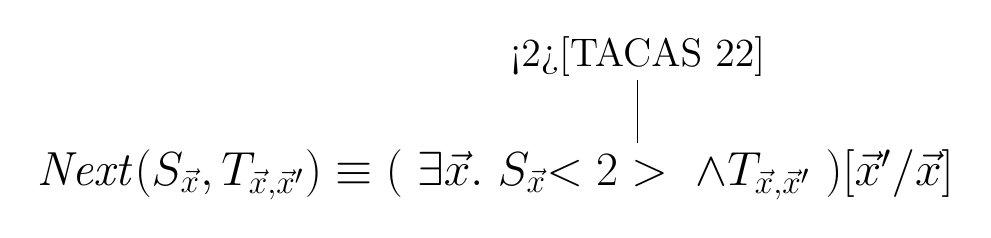
\begin{tikzpicture}
      \node at (0,0)
      {\LARGE $
        \mathit{Next}(S_{\vec{x}}, T_{\vec{x}, \vec{x}'})
        \equiv
        (
        \ \exists \vec{x} .\
        S_{\vec{x}} {\only<2>{\color{red}}\ \land} T_{\vec{x}, \vec{x}'}
        \ ) [\vec{x}' / \vec{x}]
        $};

      \onslide<2->{
        \node at ( 1.81, 1.5)
        {\Large%
          \only<2>{\color{red}}%
          [TACAS 22]%
        };

        \draw ( 1.81, 0.4) -- ++( 0.0, 0.8);
      }
    \end{tikzpicture}
  \end{center}
\end{frame}

\begin{frame}
  \frametitle{[TACAS 22]}

  \only<1>{
    \setvalue{tandem_apply  = black}
    \setvalue{tandem_reduce = black}
  }
  \only<2>{
    \setvalue{tandem_apply  = black}
    \setvalue{tandem_reduce = lightgray}
  }
  \only<3>{
    \setvalue{tandem_apply  = lightgray}
    \setvalue{tandem_reduce = black}
  }

  \begin{figure}
    \centering

    % tikz/tandem.tex (but simplified)
    \begin{tikzpicture}[scale=1.25]
      % Boxes
      \draw[color=\getvalue{tandem_apply}, thick]
        (0,0) rectangle ++(2,1)
        node[pos=.5]{\large \texttt{Apply} ($\land$)}
      ;
      \draw[color=\getvalue{tandem_reduce}, thick]
        (4,0) rectangle ++(2,1)
        node[pos=.5]{\large \texttt{Reduce}}
      ;

      % Arcs
      \draw[->, color=\getvalue{tandem_apply}, thick]
        (-0.5,0.8) -- ++(0.5,0)
        node[pos=-0.5]{\large $f$}
      ;
      \draw[->, color=\getvalue{tandem_apply}, thick]
        (-0.5,0.2) -- ++(0.5,0)
        node[pos=-0.5]{\large $g$}
      ;

      \draw[densely dashed, ->, thick] (2,0.5) -- ++(2,0)
        node[pos=0.5,above]
        {transposed}
        node[pos=0.5,below]
        {\texttt{arcs}}
      ;

      \draw[->, color=\getvalue{tandem_reduce}, thick]
        (6,0.5) -- ++(0.5,0)
        node[pos=2.0]{\large $f \land g$}
      ;
    \end{tikzpicture}
  \end{figure}
\end{frame}

\begin{frame}[plain,noframenumbering]
  \begin{center}
    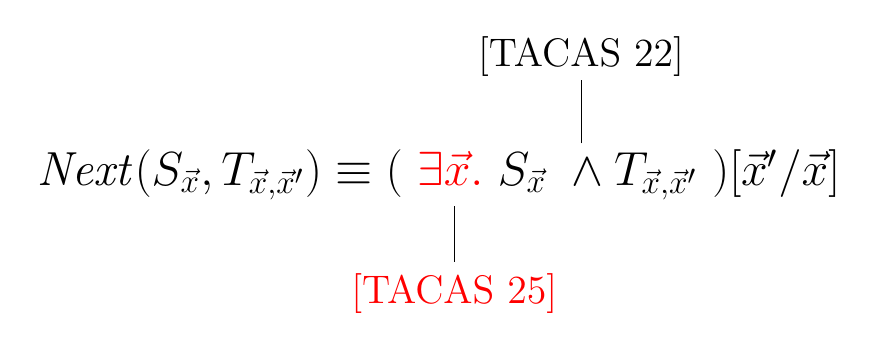
\begin{tikzpicture}
      \node at (0,0)
      {\LARGE $
        \mathit{Next}(S_{\vec{x}}, T_{\vec{x}, \vec{x}'})
        \equiv
        (
        \ {\color{red} \exists \vec{x} .}\
        S_{\vec{x}} \ \land T_{\vec{x}, \vec{x}'}
        \ ) [\vec{x}' / \vec{x}]
        $};

      {
        \node at ( 1.81, 1.5)
        {\Large%
          [TACAS 22]%
        };

        \draw ( 1.81, 0.4) -- ++( 0.0, 0.8);
      }

      {
        \node at (0.2,-1.5)
        {\Large%
          \color{red}%
          [TACAS 25]%
        };

        \draw (0.2,-0.4) -- ++(0,-0.7);
      }
    \end{tikzpicture}
  \end{center}
\end{frame}

\begin{frame}
  \frametitle{[TACAS 25]}

  \begin{figure}
    \centering
    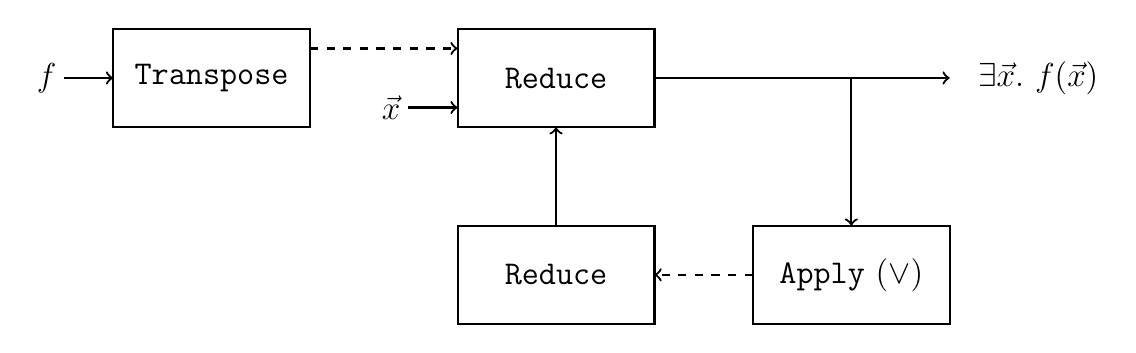
\begin{tikzpicture}[scale=1.25]
      % Boxes (outer)
      \draw[thick] (0,0) rectangle ++(2,1)
      node[pos=.5]{\large \texttt{Transpose}};

      \draw[thick] (3.5,0) rectangle ++(2,1)
      node[pos=.5]{\large \texttt{Reduce}};

      % Arcs (outer)
      \draw[->, thick] (-0.5,0.5) -- ++(0.5,0)
      node[pos=-0.35]{\large $f$};

      \draw[->, thick, dashed] (2,0.8) -- ++(1.5,0);

      \draw[->, thick] ( 3.0,0.2) -- ++(0.5,0)
      node[pos=-0.35]{\large $\vec{x}$};

      \draw[->, thick] (5.5,0.5) -- ++(3,0)
      node[pos=1.3]{\large $\exists \vec{x}.\ f(\vec{x})$};

      % Boxes (inner)
      \draw[thick] (6.5,-2) rectangle ++(2,1)
      node[pos=.5]{\large \texttt{Apply} ($\lor$)};
      \draw[thick] (3.5,-2) rectangle ++(2,1)
      node[pos=.5]{\large \texttt{Reduce}};

      % Arcs (inner)
      \draw[->, thick] (7.5,0.5) -- ++(0,-1.5);

      \draw[->, thick, dashed] (6.5,-1.5) -- ++(-1.0,0);

      \draw[->, thick] (4.5,-1) -- ++(0,1);
    \end{tikzpicture}
  \end{figure}
\end{frame}

\begin{frame}[plain,noframenumbering]
  \begin{center}
    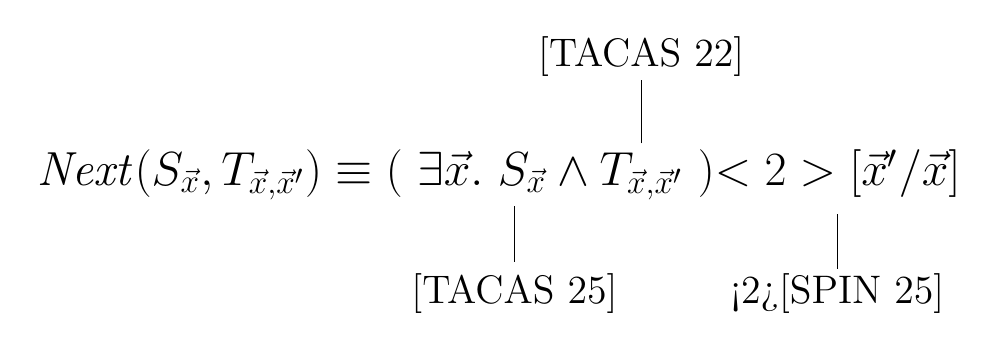
\begin{tikzpicture}
      \node at (0,0)
      {\LARGE $
        \mathit{Next}(S_{\vec{x}}, T_{\vec{x}, \vec{x}'})
        \equiv
        (
        \ \exists \vec{x} .\
        S_{\vec{x}} \land T_{\vec{x}, \vec{x}'}
        \ ) {\only<2>{\color{red}}[\vec{x}' / \vec{x}]}
        $};

      {
        \node at ( 1.81, 1.5)
        {\Large%
          [TACAS 22]%
        };

        \draw ( 1.81, 0.4) -- ++( 0, 0.8);
      }

      {
        \node at (0.2,-1.5)
        {\Large%
          [TACAS 25]%
        };

        \draw (0.2,-0.4) -- ++(0,-0.7);
      }

      \onslide<2->{
        \node at (4.3,-1.5)
        {\Large%
          \only<2>{\color{red}}%
          [SPIN 25]%
        };

        \draw ( 4.3,-0.5) -- ++(0,-0.7);
      }
    \end{tikzpicture}
  \end{center}
\end{frame}

\begin{frame}
  \frametitle{Replace}

  \begin{definition}
    A relabelling $\pi$ is monotonic if $x_i < x_j \implies \pi(x_i) < \pi(x_j)$
  \end{definition}

  \begin{lemma}
    If $\pi$ is monotonic, then the BDD $f(\vec{x})$ is isomorphic to $f(\pi(\vec{x}))$.
  \end{lemma}

  \medskip

  \begin{itemize}
  \item<2-> {\bf One can apply $\pi$ in a single linear scan.}

    $\Oh{N}$ time, $2 \cdot \scan{N}$ I/Os, and $N$ external space.

  \item<3-> {\bf One can incorporate $\pi$ into a (succeeding) top-down \texttt{Apply} sweep.}

    $\Oh{N}$ time, $0$ I/Os, and $0$ external space.

  \item<3-> {\bf One can incorporate $\pi$ into a (preceeding) bottom-up \texttt{Reduce} sweep.}

    $\Oh{n}$ time, $0$ I/Os, and $0$ external space.
  \end{itemize}
\end{frame}

\begin{frame}[t]
  \frametitle{AndExists}

  \begin{block}{Observation}
    The I/O-efficient \texttt{And} [TACAS 22] and \texttt{Exists} [TACAS 25] operations can be merged:
  \end{block}

  \only<1-2>{
    \begin{figure}[y]
      \centering

      \begin{tikzpicture}
        % -----------------------------------------------
        % And
        \draw[thick] (-3,-2) rectangle ++(2,1)
        node[pos=.5]{\texttt{Apply} ($\land$)};

        \draw[->, thick] (-3.5,-1.5) -- ++(0.5,0)
        node[pos=-0.55]{\large $f$};

        \only<1>{
          \draw[thick] (0,-2) rectangle ++(2,1)
          node[pos=.5]{\texttt{Reduce}};

          \draw[->, thick, dashed] (-1.0,-1.5) -- ++(1,0);
          \draw[->, thick] (1.0,-1.0) -- ++(0,1);
        }
        \only<2>{
          \draw[thick, lightgray] (0,-2) rectangle ++(2,1)
          node[pos=.5]{\texttt{Reduce}};
        }

        % -----------------------------------------------
        % Exists (outer)
        \only<1>{
          \draw[thick] (0,0) rectangle ++(2,1)
          node[pos=.5]{\texttt{Transpose}};
        }
        \only<2>{
          \draw[thick, lightgray] (0,0) rectangle ++(2,1)
          node[pos=.5]{\texttt{Transpose}};
        }

        \draw[thick] (3.5,0) rectangle ++(2,1)
        node[pos=.5]{\texttt{Reduce}};

        % Arcs (outer)
        \only<1>{
          \draw[->, thick, dashed] (2,0.8) -- ++(1.5,0);
        }
        \only<2>{
          \draw[->, thick, dashed] (-1.0,-1.5) -- ++(0.5,0) -- ++(0,1) -- ++(2.8,0) -- ++(0,1.3) -- ++(1.2,0);
        }

        \draw[->, thick] ( 3.0,0.2) -- ++(0.5,0)
        node[pos=-0.55]{$\vec{x}$};

        \draw[->, thick] (5.5,0.5) -- ++(2,0)
        node[pos=1.5]{$\exists \vec{x}.\ f(\vec{x})$};

        % Boxes (inner)
        \draw[thick] (6,-2) rectangle ++(2,1)
        node[pos=.5]{\texttt{Apply} ($\lor$)};
        \draw[thick] (3.5,-2) rectangle ++(2,1)
        node[pos=.5]{\texttt{Reduce}};

        % Arcs (inner)
        \draw[->, thick] (7,0.5) -- ++(0,-1.5);

        \draw[->, thick, dashed] (6,-1.5) -- ++(-0.5,0);

        \draw[->, thick] (4.5,-1) -- ++(0,1);
      \end{tikzpicture}
    \end{figure}
  }
  \only<3->{
    \begin{itemize}
    \item<3-> {\bf The outer accumulating \texttt{Reduce} sweep of the \texttt{Exists} can do double-duty
        as the \texttt{Reduce} sweep of the preceeding \texttt{And} operation.}

      This saves $\Theta(\sort{N})$ time and I/Os.

      \medskip

    \item<4-> {\bf The \texttt{And} operation can prune subtrees that trivially will become redundant
        during the succeeding \texttt{Exists}.}

      This can save up to $\Oh{\sort{N^{2^k}}}$ time and I/Os.

      In practice, this only saves up to $\Oh{\sort{N}}$ time and I/Os.
    \end{itemize}
  }
\end{frame}

\blankframe

\begin{frame}
  \frametitle{Experiment: Next($S_{\vec{x}}, T_{\vec{x}, \vec{x}'}$)}

  \begin{figure}
    \centering

    \begin{subfigure}{0.3\linewidth}
      \centering

      \begin{tikzpicture}
        \begin{axis}[%
          width=1.05\linewidth, height=1.2\linewidth,
          every tick label/.append style={font=\scriptsize},
          % x-axis
          xlabel={\scriptsize Memory (GiB)},
          xmin=0.8,
          xtick={1,2,4,8},
          xticklabels={1,2,4,8},
          xmax=10,
          xmode=log,
          % y-axis
          ylabel={\scriptsize Running Time (s)},
          ymin=100,
          ymax=43200,
          ytick={100,1000,10000,100000},
          ymode=log,
          % grid
          grid style={dashed,black!12},
          ]

          % BuDDy memory out
          % \addplot+ [style=x_buddy, forget plot] coordinates {
          % (2, 36000)
          % };

          %   data
          \addplot+ [style=plot_adiar]
          table {./data/memory.gpufp_20_a.adiar.tex};

          \addplot+ [style=plot_buddy]
          table {./data/memory.gpufp_20_a.buddy.tex};
        \end{axis}
      \end{tikzpicture}

      \caption{\tiny \texttt{GPUForwardProgress}~20a}
    \end{subfigure}
    \hspace{-30pt}
    \begin{subfigure}{0.3\linewidth}
      \centering

      \begin{tikzpicture}
        \begin{axis}[%
          width=1.05\linewidth, height=1.2\linewidth,
          every tick label/.append style={font=\scriptsize},
          % x-axis
          xlabel={\scriptsize Memory (GiB)},
          xmin=0.8,
          xtick={1,2,4,8},
          xticklabels={1,2,4,8},
          xmax=10,
          xmode=log,
          % y-axis
          ymin=100,
          ymax=43200,
          ytick={100,1000,10000,100000},
          yticklabels={,,,},
          ymode=log,
          % grid
          grid style={dashed,black!12},
          ]

          % BuDDy memory out
          % \addplot+ [style=x_buddy, forget plot] coordinates {
          % (2, 36000)
          % };

          %   data
          \addplot+ [style=plot_adiar]
          table {./data/memory.smhome_16.adiar.tex};

          \addplot+ [style=plot_buddy]
          table {./data/memory.smhome_16.buddy.tex};
        \end{axis}
      \end{tikzpicture}

      \caption{\tiny \texttt{SmartHome}~16}
    \end{subfigure}
    \hspace{-36.8pt}
    \begin{subfigure}{0.5\linewidth}
      \centering

      \begin{tikzpicture}
        \begin{axis}[%
          width=1.1\linewidth, height=0.72\linewidth,
          every tick label/.append style={font=\scriptsize},
          % x-axis
          xlabel={\scriptsize Memory (GiB)},
          xmin=0.8,
          xtick={1,2,4,8,16,32,64},
          xticklabels={1,2,4,8,16,32,64},
          xmax=80,
          xmode=log,
          % y-axis
          ymin=100,
          ymax=43200,
          ytick={100,1000,10000,100000},
          yticklabels={,,,},
          ymode=log,
          % grid
          grid style={dashed,black!12},
          ]

          % BuDDy time out
          \addplot+ [style=x_buddy, forget plot] coordinates {
            (2, 36000)
            (4, 36000)
            (8, 36000)
          };

          % data
          \addplot+ [style=plot_adiar]
          table {./data/memory.shield_s_ppp_010_a.adiar.tex};

          \addplot+ [style=plot_buddy]
          table {./data/memory.shield_s_ppp_010_a.buddy.tex};
        \end{axis}
      \end{tikzpicture}

      \caption{\tiny \texttt{ShieldPPPs}~10a}
    \end{subfigure}

    \smallskip

    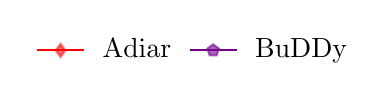
\begin{tikzpicture}
      \begin{customlegend}[
        legend columns=-1,
        legend style={draw=none,column sep=1ex},
        legend entries={
          Adiar,
          BuDDy
        }
        ]
        \addlegendimage{style=plot_adiar}
        \addlegendimage{style=plot_buddy}
      \end{customlegend}
    \end{tikzpicture}

    \caption{Relational Product for MCC models with a $2^{25}$ state space BDD. Timeouts are marked
      as stars.}
  \end{figure}
\end{frame}

\begin{frame}
  \frametitle{Experiment: Next($S_{\vec{x}}, T_{\vec{x}, \vec{x}'}$) \& Prev($S_{\vec{x}}, T_{\vec{x}, \vec{x}'}$)}

  \begin{figure}
    \centering

    \begin{subfigure}{0.49\linewidth}
      \centering

      \begin{tikzpicture}
        \begin{axis}[%
          width=1\linewidth, height=0.696\linewidth,
          every tick label/.append style={font=\scriptsize},
          % x-axis
          xlabel={\scriptsize Other (s)},
          xmin=10,
          xtick={10,100,1000,10000,100000},
          xmax=100000,
          xmode=log,
          % y-axis
          ylabel={\scriptsize Adiar (s)},
          ymin=10,
          ymax=100000,
          ytick={1,10,100,1000,10000,100000},
          ymode=log,
          % grid
          grid style={dashed,black!12},
          ]

          % x lines
          \addplot[domain=10:100000, samples=8, color=black, dotted]
          {0.01*x};
          \addplot[domain=10:100000, samples=8, color=black, dashed]
          {0.1*x};
          \addplot[domain=10:100000, samples=8, color=black]
          {x};
          \addplot[domain=10:10000, samples=8, color=black, dashed]
          {10*x};
          \addplot[domain=10:1000, samples=8, color=black, dotted]
          {100*x};

          % data
          \addplot+ [style=dots_buddy]
          table {./data/next.buddy.tex};

          \addplot+ [style=dots_cal]
          table {./data/next.cal.tex};

          \addplot+ [style=dots_cudd]
          table {./data/next.cudd.tex};

          \addplot+ [style=dots_libbdd]
          table {./data/next.libbdd.tex};
        \end{axis}
      \end{tikzpicture}

      \caption{Next($S_{\vec{x}}, T_{\vec{x}, \vec{x}'}$)}
    \end{subfigure}
    \begin{subfigure}{0.49\linewidth}
      \centering

      \begin{tikzpicture}
        \begin{axis}[%
          width=1\linewidth, height=0.696\linewidth,
          every tick label/.append style={font=\scriptsize},
          % x-axis
          xlabel={\scriptsize Other (s)},
          xmin=10,
          xtick={1,10,100,1000,10000,100000},
          xmax=100000,
          xmode=log,
          % y-axis
          ymin=10,
          ymax=100000,
          ytick={1,10,100,1000,10000,100000},
          yticklabels={,,,,,},
          ymode=log,
          % grid
          grid style={dashed,black!12},
          ]

          % x lines
          \addplot[domain=10:100000, samples=8, color=black, dotted]
          {0.01*x};
          \addplot[domain=10:100000, samples=8, color=black, dashed]
          {0.1*x};
          \addplot[domain=10:100000, samples=8, color=black]
          {x};
          \addplot[domain=10:10000, samples=8, color=black, dashed]
          {10*x};
          \addplot[domain=10:1000, samples=8, color=black, dotted]
          {100*x};

          % data
          \addplot+ [style=dots_buddy]
          table {./data/prev.buddy.tex};

          \addplot+ [style=dots_cal]
          table {./data/prev.cal.tex};

          \addplot+ [style=dots_cudd]
          table {./data/prev.cudd.tex};

          \addplot+ [style=dots_libbdd]
          table {./data/prev.libbdd.tex};
        \end{axis}
      \end{tikzpicture}

      \caption{Prev($S_{\vec{x}}, T_{\vec{x}, \vec{x}'}$)}
    \end{subfigure}

    
\begin{tikzpicture}
      \begin{customlegend}[
        legend columns=-1,
        legend style={draw=none,column sep=1ex},
        legend entries={
          BuDDy,
          CAL,
          CUDD,
          LibBDD
        }
        ]
        \addlegendimage{style=dots_buddy}
        \addlegendimage{style=dots_cal}
        \addlegendimage{style=dots_cudd}
        \addlegendimage{style=dots_libbdd}
      \end{customlegend}
    \end{tikzpicture}

    \caption{Relational Product for MCC models, $384$~GiB of memory, and $2^{22}, \dots, 2^{25}$
      state space BDDs.}
  \end{figure}
\end{frame}

\begin{frame}
  \frametitle{Experiment: Reachability}

  \begin{figure}
    \centering

    \begin{tikzpicture}
      \begin{axis}[%
        width=1\linewidth, height=0.405\linewidth,
        every tick label/.append style={font=\scriptsize},
        % x-axis
        xlabel={\scriptsize Other (s)},
        xmin=0.001,
        xtick={0.001,0.01,0.1,1,10,100,1000,10000},
        xmax=20000,
        xmode=log,
        % y-axis
        ylabel={\scriptsize Adiar (s)},
        ymin=0.001,
        ymax=10000,
        ytick={0.001,0.01,0.1,1,10,100,1000,10000},
        ymode=log,
        % grid
        grid style={dashed,black!12},
        ]

        % x lines
        \addplot[domain=0.001:20000, samples=8, color=black, dotted]
        {0.01*x};
        \addplot[domain=0.001:20000, samples=8, color=black, dashed]
        {0.1*x};
        \addplot[domain=0.001:10000, samples=8, color=black]
        {x};
        \addplot[domain=0.001:1000, samples=8, color=black, dashed]
        {10*x};
        \addplot[domain=0.001:100, samples=8, color=black, dotted]
        {100*x};

        % data
        \addplot+ [style=dots_buddy]
        table {./data/reachability.buddy.tex};

        \addplot+ [style=dots_cal]
        table {./data/reachability.cal.tex};

        \addplot+ [style=dots_cudd]
        table {./data/reachability.cudd.tex};

        \addplot+ [style=dots_libbdd]
        table {./data/reachability.libbdd.tex};

        \addplot+ [style=dots_sylvan]
        table {./data/reachability.sylvan.tex};
      \end{axis}
    \end{tikzpicture}

    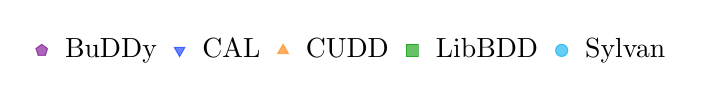
\begin{tikzpicture}
      \begin{customlegend}[
        legend columns=-1,
        legend style={draw=none,column sep=1ex},
        legend entries={
          BuDDy,
          CAL,
          CUDD,
          LibBDD,
          Sylvan
        }
        ]
        \addlegendimage{style=dots_buddy}
        \addlegendimage{style=dots_cal}
        \addlegendimage{style=dots_cudd}
        \addlegendimage{style=dots_libbdd}
        \addlegendimage{style=dots_sylvan}
      \end{customlegend}
    \end{tikzpicture}

    \caption{16 Petri Nets [MCC 21--23] with $384$~GiB of memory.}
  \end{figure}
\end{frame}

\begin{frame}
  \frametitle{Experiment: Deadlock Detection}

  \begin{figure}
    \centering

    \begin{tikzpicture}
      \begin{axis}[%
        width=1\linewidth, height=0.405\linewidth,
        every tick label/.append style={font=\scriptsize},
        % x-axis
        xlabel={\scriptsize Other (s)},
        xmin=0.001,
        xtick={0.001,0.01,0.1,1,10,100,1000,10000,100000},
        xmax=20000,
        xmode=log,
        % y-axis
        ylabel={\scriptsize Adiar (s)},
        ymin=0.001,
        ymax=1000,
        ytick={0.001,0.01,0.1,1,10,100,1000},
        ymode=log,
        % grid
        grid style={dashed,black!12},
        ]

        % x lines
        \addplot[domain=0.001:100000, samples=8, color=black, dotted]
        {0.01*x};
        \addplot[domain=0.001:100000, samples=8, color=black, dashed]
        {0.1*x};
        \addplot[domain=0.001:1000, samples=8, color=black]
        {x};
        \addplot[domain=0.001:100, samples=8, color=black, dashed]
        {10*x};
        \addplot[domain=0.001:10, samples=8, color=black, dotted]
        {100*x};

        % data
        \addplot+ [style=dots_buddy]
        table {./data/deadlock.buddy.tex};

        \addplot+ [style=dots_cal]
        table {./data/deadlock.cal.tex};

        \addplot+ [style=dots_cudd]
        table {./data/deadlock.cudd.tex};

        \addplot+ [style=dots_libbdd]
        table {./data/deadlock.libbdd.tex};

        \addplot+ [style=dots_sylvan]
        table {./data/deadlock.sylvan.tex};
      \end{axis}
    \end{tikzpicture}

    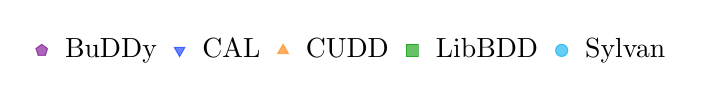
\begin{tikzpicture}
      \begin{customlegend}[
        legend columns=-1,
        legend style={draw=none,column sep=1ex},
        legend entries={
          BuDDy,
          CAL,
          CUDD,
          LibBDD,
          Sylvan
        }
        ]
        \addlegendimage{style=dots_buddy}
        \addlegendimage{style=dots_cal}
        \addlegendimage{style=dots_cudd}
        \addlegendimage{style=dots_libbdd}
        \addlegendimage{style=dots_sylvan}
      \end{customlegend}
    \end{tikzpicture}

    \caption{16 Petri Nets [MCC 21--23] and 59 Boolean Networks [AEON, PyBoolNet] with $384$~GiB RAM.}
  \end{figure}
\end{frame}

\begin{frame}
  \frametitle{Experiment: SCC Decomposition}

  \begin{figure}
    \centering

    \vspace{4.5pt}

    \begin{tikzpicture}
      \begin{axis}[%
        width=1\linewidth, height=0.405\linewidth,
        every tick label/.append style={font=\scriptsize},
        % x-axis
        xlabel={\scriptsize Other (s)},
        xmin=0.001,
        xtick={0.001,0.01,0.1,1,10,100,1000,10000,100000},
        xmax=200000,
        xmode=log,
        % y-axis
        ylabel={\scriptsize Adiar (s)},
        ymin=0.001,
        ymax=200000,
        ytick={0.001,0.01,0.1,1,10,100,1000,10000,100000},
        ymode=log,
        % grid
        grid style={dashed,black!12},
        ]

        % x lines
        \addplot[domain=0.001:200000, samples=8, color=black, dotted]
        {0.01*x};
        \addplot[domain=0.001:200000, samples=8, color=black, dashed]
        {0.1*x};
        \addplot[domain=0.001:200000, samples=8, color=black]
        {x};
        \addplot[domain=0.001:20000, samples=8, color=black, dashed]
        {10*x};
        \addplot[domain=0.001:2000, samples=8, color=black, dotted]
        {100*x};

        % data
        \addplot+ [style=dots_buddy]
        table {./data/scc.buddy.tex};

        \addplot+ [style=dots_cal]
        table {./data/scc.cal.tex};

        \addplot+ [style=dots_cudd]
        table {./data/scc.cudd.tex};

        \addplot+ [style=dots_libbdd]
        table {./data/scc.libbdd.tex};

        \addplot+ [style=dots_sylvan]
        table {./data/scc.sylvan.tex};
      \end{axis}
    \end{tikzpicture}

    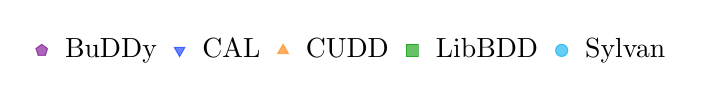
\begin{tikzpicture}
      \begin{customlegend}[
        legend columns=-1,
        legend style={draw=none,column sep=1ex},
        legend entries={
          BuDDy,
          CAL,
          CUDD,
          LibBDD,
          Sylvan
        }
        ]
        \addlegendimage{style=dots_buddy}
        \addlegendimage{style=dots_cal}
        \addlegendimage{style=dots_cudd}
        \addlegendimage{style=dots_libbdd}
        \addlegendimage{style=dots_sylvan}
      \end{customlegend}
    \end{tikzpicture}

    \caption{16 Petri Nets [MCC 21--23] and 59 Boolean Networks [AEON, PyBoolNet] with $384$~GiB RAM.}
  \end{figure}
\end{frame}

\begin{frame}
  \frametitle{Conclusions and Future Work}

  \begin{itemize}
  \item<1-> {\bf To improve the I/O-efficient \emph{Next}($S_{\vec{x}}, T_{\vec{x}, \vec{x'}}$), focus
      on \emph{AndExists}.}

    \begin{itemize}
      \small

    \item Factor of $\sim 2\times$ by using a \texttt{AndExists} instead of \texttt{And} and
      \texttt{Exists} for conventional depth-first implementations \footnote{\tiny\quad Van Dijk et
        al.: \emph{A Comparative Study of BDD packages for Probabilistic Symbolic Model Checking}.
        (2015)}. This may explain the sudden performance gap.

    \item For larger instances, less than $\tfrac{1}{10}$th of the time is spent on the \texttt{And}.
    \end{itemize}

  \item<2-> {\bf Deal with small BDDs using Depth-first Recursion.}

  \item<3-> {\bf Apply ideas from recent and more advanced BDD algorithms.}

    {\small

      For example the ones in \footnote{\tiny\quad Van Dijk: \emph{Sylvan – Multi-core Decision
          Diagrams}. (2016)}, %
      \footnote{\tiny\quad Van Dijk et al.: \emph{Multi-core on-the-fly saturation}. (2019)}, %
      \footnote{\tiny\quad Brand et al.: \emph{A Decision Diagram Operation for Reachability}.
        (2023).}, and %
      \footnote{\tiny\quad Marmorstein \& Siminiceanu: \emph{The Saturation algorithm for Symbolic
          State-space Exploration}. (2006).} .}

    \bigskip

  \item<4-> {\bf Design a \emph{Replace}($\pi$) for Non-monotone Variable Substitutions.}
  \end{itemize}

  \bigskip
\end{frame}

\begin{frame}[plain,noframenumbering]
  {\Large \textbf{Steffan Christ Sølvsten}}
  \vspace{1pt} {\hrule width0.45\linewidth}

  \vspace{5pt}

  \begin{itemize}
  \item[\faIcon{envelope}] \mailto{soelvsten@cs.au.dk}
  \item[\faIcon{twitter}] \href{https://www.twitter.com/ssoelvsten}{@ssoelvsten}
  \end{itemize}

  \vspace{10pt}

  {\Large \textbf{Adiar}}
  \vspace{1pt} {\hrule width0.45\linewidth}

  \vspace{5pt}

  \begin{itemize}
  \item[\faIcon{code}]
    \href{http://github.com/ssoelvsten/adiar}{github.com/ssoelvsten/adiar}
  \item[\faIcon{book}\hspace{2pt}]
    \href{http://ssoelvsten.github.io/adiar}{ssoelvsten.github.io/adiar}
  \end{itemize}


  \vspace{10pt}

  \includegraphics[width=0.2\linewidth]{../external/aulogo_uk_var2_black.eps}
\end{frame}

\begin{frame}
  \begin{figure}
    \centering

    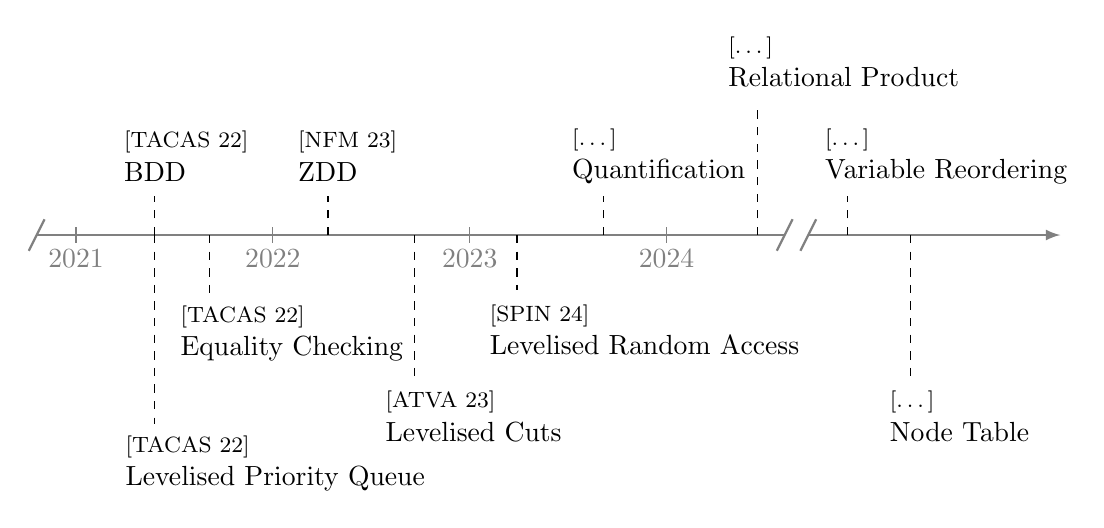
\begin{tikzpicture}
      % PhD line
\draw[gray][thick] (0.6,0.2) -- (0.4,-0.2);
\draw[gray][-, thick] (0.5,0) -- (10,0);
\draw[gray][thick] (10.1,0.2) -- (9.9,-0.2);

% 2021
\draw[gray] (1,-0.1) -- ++(0,0.2);
\node[gray] at (1,-0.3) {$2021$};

\draw[dashed, color=black] (2,0) -- ++(0,0.5);
\node[color=black, align=left] at (2.4,1.0)
{\footnotesize [TACAS 22]\\BDD};

\draw[dashed, color=black] (2,0) -- ++(0,-2.4);
\node[color=black, align=left] at (3.53,-2.9)
{\footnotesize [TACAS 22]\\Levelised Priority Queue};

\draw[dashed, color=black] (2.7,0) -- ++(0,-0.8);
\node[color=black, align=left] at (3.74,-1.25)
{\footnotesize [TACAS 22]\\Equality Checking};

% 2022
\draw[gray] (3.5,-0.1) -- ++(0,0.2);
\node[gray] at (3.5,-0.3) {$2022$};

\draw[dashed, color=black] (4.2,0) -- ++(0,0.5);
\node[color=black, align=left] at (4.45,1.0)
{\footnotesize [NFM 23]\\ZDD};

\draw[dashed, color=black] (5.3,0) -- ++(0,-1.8);
\node[color=black, align=left] at (6.05,-2.3)
{\footnotesize [ATVA 23]\\Levelised Cuts};

% 2023
\draw[gray] (6,-0.1) -- ++(0,0.2);
\node[gray] at (6,-0.3) {$2023$};

\draw[dashed, color=black] (6.6,0) -- ++(0,-0.7);
\node[color=black, align=left] at (8.22,-1.2)
{\footnotesize [SPIN 24]\\Levelised Random Access};

\draw[dashed, color=black] (7.7,0) -- ++(0,0.5);
\node[color=black, align=left] at (8.4,1.0)
{\footnotesize [\dots]\\Quantification};

% 2024
\draw[gray] (8.5,-0.1) -- ++(0,0.2);
\node[gray] at (8.5,-0.3) (y2024) {$2024$};

\draw[dashed, color=black] (9.65,0) -- ++(0,1.6);
\node[color=black, align=left] at (10.75,2.2)
{\footnotesize [\dots]\\Relational Product};

% 2025
%\draw[gray] (11,-0.1) -- ++(0,0.2);
%\node[gray] at (11,-0.3) (y2025) {$2025$};

% PostDoc (?) line
\draw[gray][thick] (10.4,0.2) -- (10.2,-0.2);
\draw[gray][-latex, thick] (10.3,0) -- (13.5,0);

% PostDoc (?)

\draw[dashed, color=black] (10.8,0) -- ++(0,0.5);
\node[color=black, align=left] at (12.05,1.0)
{\footnotesize [\dots]\\Variable Reordering};

\draw[dashed, color=black] (11.6,0) -- ++(0,-1.8);
\node[color=black, align=left] at (12.22,-2.3)
{\footnotesize [\dots]\\Node Table};

    \end{tikzpicture}
  \end{figure}
\end{frame}

\end{document}
